% !TeX root = ../main.tex

\chapter{MBDP算法在决策控制任务中的应用}

\section{Mujoco控制任务}

在本课题中,为了证明上述改进方案的可行性,以及验证改进效果,本课题通过实验初步验证了2个问题:

\begin{itemize}
    \item 改进后的算法在强化学习的标准测试任务上相比最新的算法提升如何?
    \item 是否能达到\ref{sec:rollout-method}节中所描述的可以通过动态调整参数$\alpha,\beta$来取得不同决策策略的效果?
\end{itemize}

本课题使用强化学习中广泛使用的标准测试环境MuJoCo模拟器\cite{todorov2012mujoco}进行实验,首先在四组不同任务上,与最新的MBPO \cite{janner2019trust}算法、STEVE \cite{buckman2018sample}算法、SLBO \cite{Luo2019AlgorithmicGuarantees}算法以及无模型的SAC \cite{haarnoja2018soft}算法进行对比实验。在本课题的算法中,使用了参数$\alpha=0.5, \beta=0.85$。对比实验结果如图\ref{fig:performance}所示,其中横轴为训练的步数,纵轴为相应步数对应的平均收益。图中实线为不同随机种子实验的均值结果,阴影区域则表示这些实验的方差。由于SAC是无模型强化学习算法,相较基于模型的强化学习算法收敛速度较慢,因此只在图中画出部分训练曲线图,其最终收敛值通过虚线标注出来。

根据实验结果可以看出,本课题设计的改进算法在四种不同的任务环境中,均有着超越现有算法的表现。

\begin{figure}
  \centering
  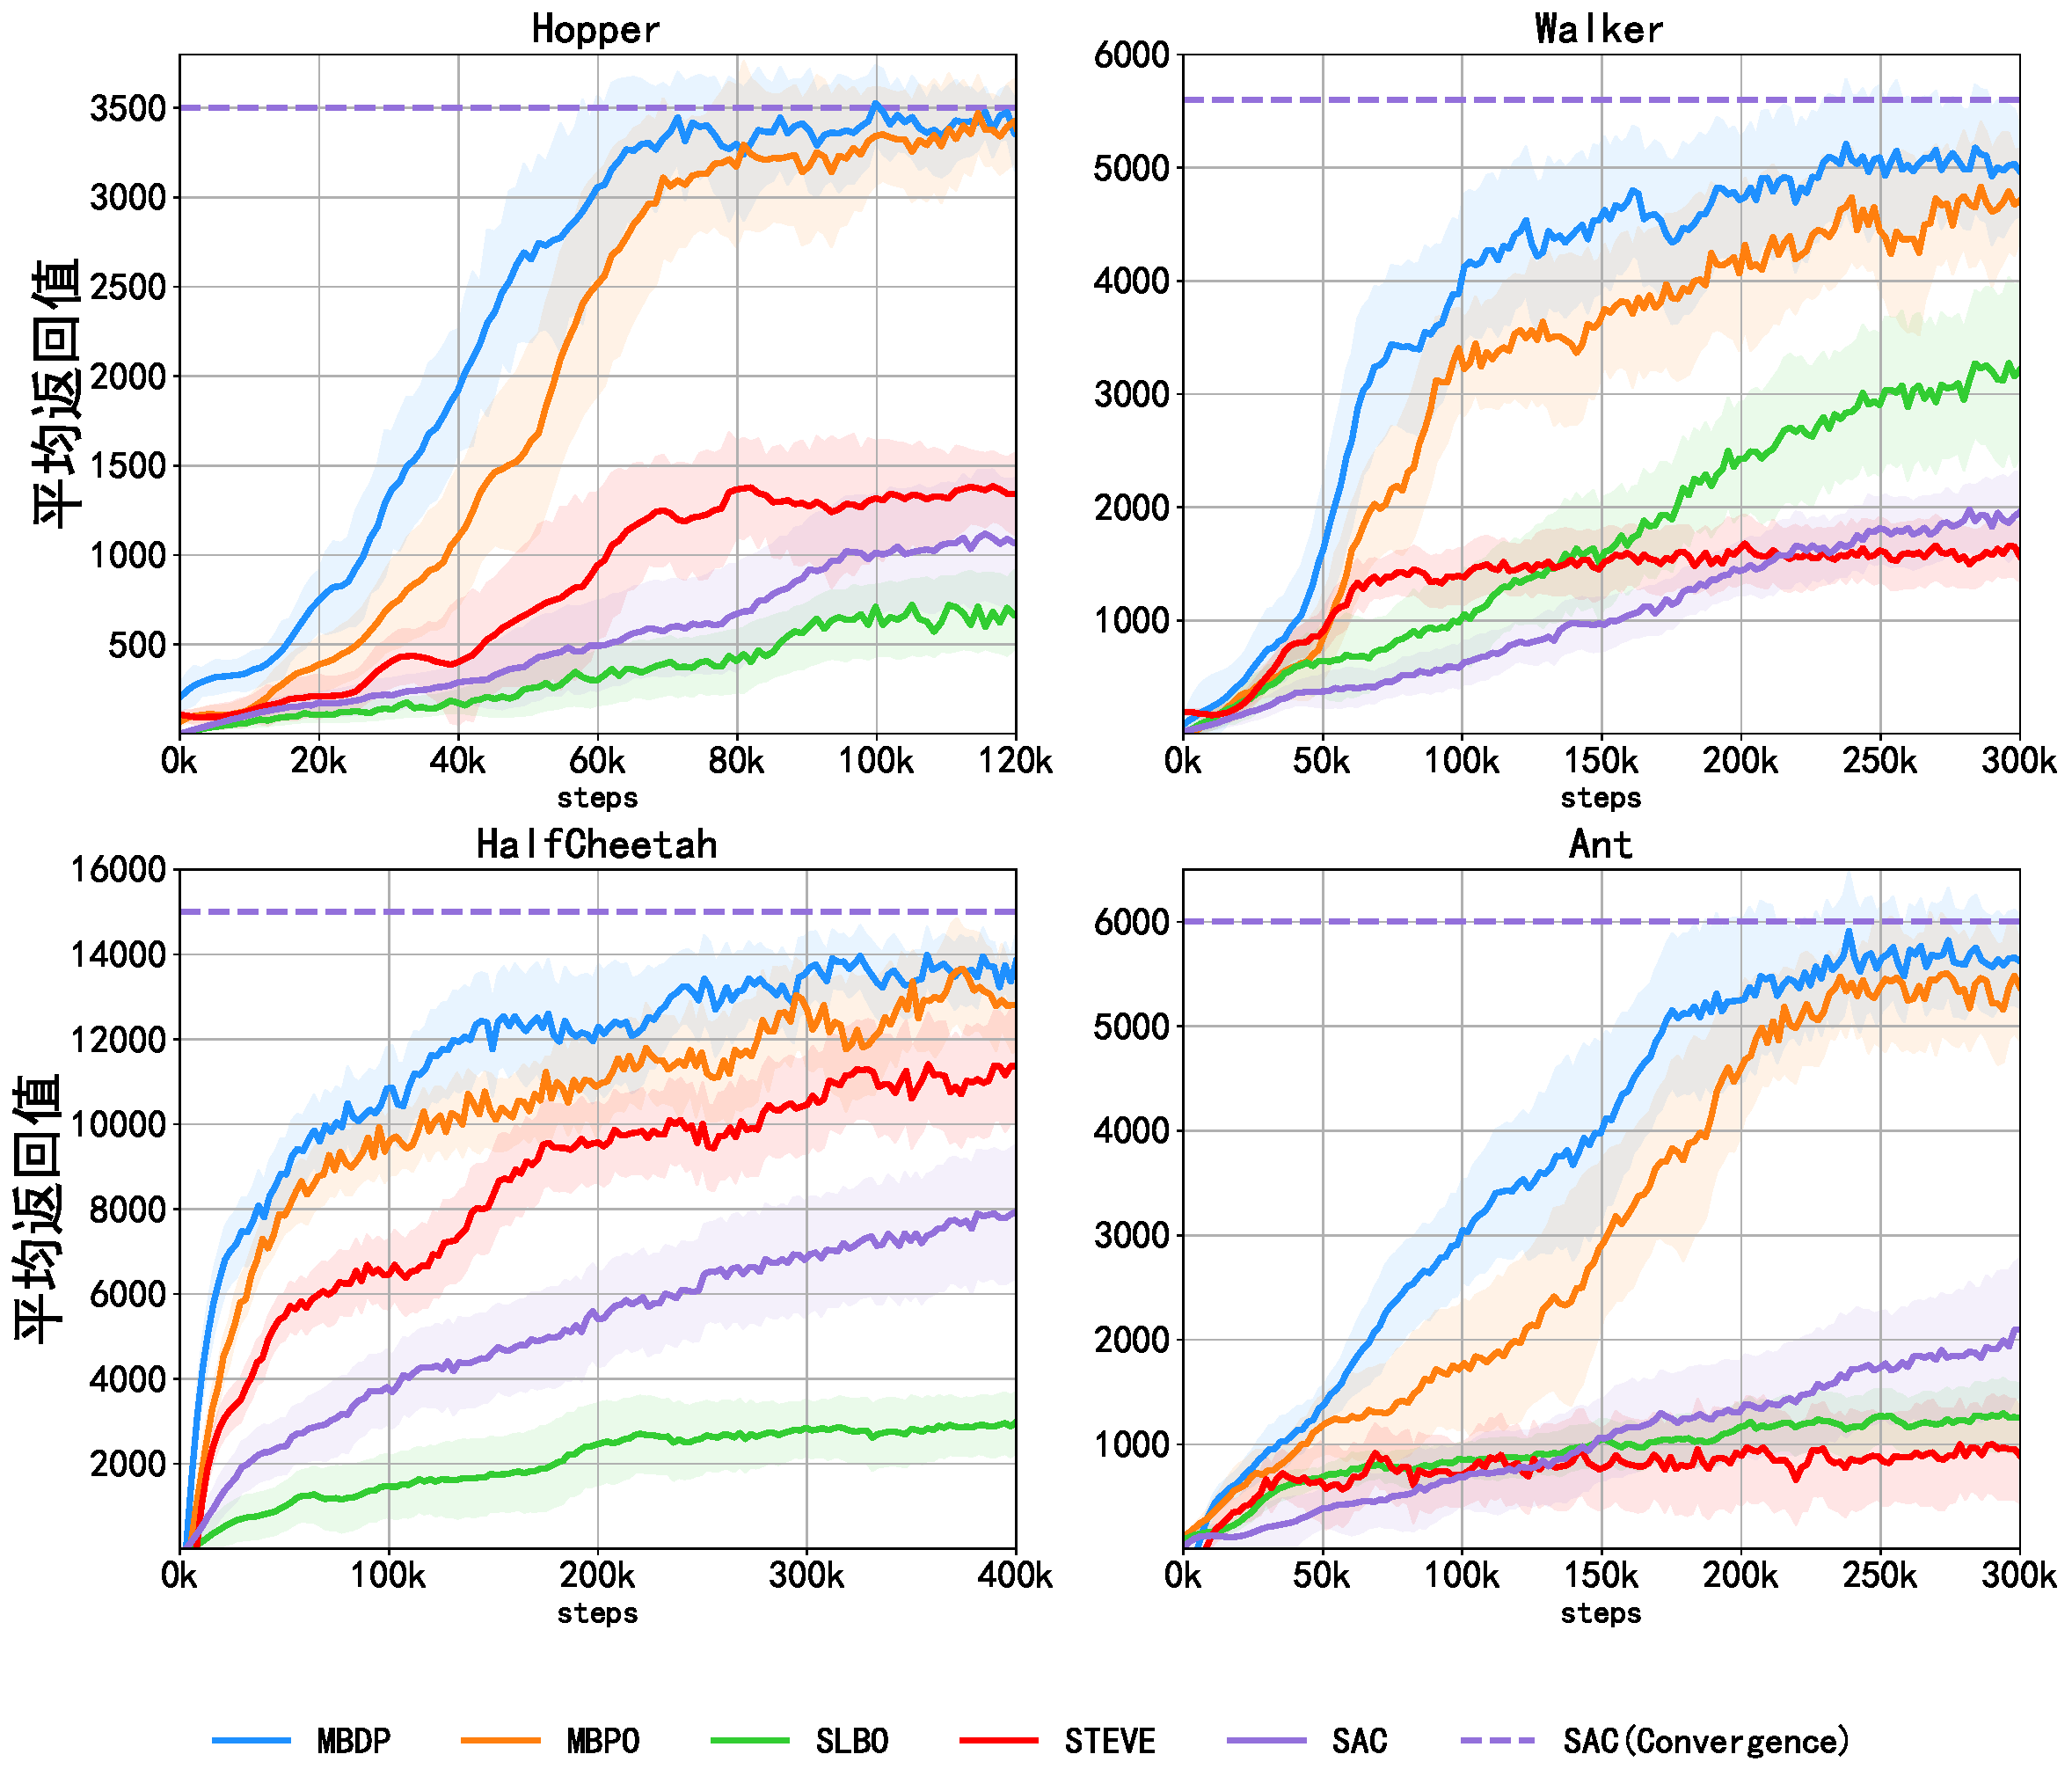
\includegraphics[width=0.9\textwidth]{figures/performance.pdf}
  \caption{各算法在不同任务下的训练曲线图。}
  \label{fig:performance}
\end{figure}

为了进一步验证改进算法的鲁棒性提升,对实验环境加入了不同程度的干扰,本课题在Hopper和HalfCheetah两个任务环境下,将物体的质量和摩擦系数均加以数值区间为$[0.5,1.5]$的干扰,同时以最新的MBPO算法作为对照标准进行对比实验。在各组干扰条件下均进行了一组实验,Hopper任务中每组实验训练$3\times 10^5$轮,HalfCheetah任务中每组任务训练$6\times 10^5$轮,实验结果以热力图的形式绘制成图\ref{fig:robustness-heatmap},其中每一个方格表示一组干扰系数下训练相应轮数后的收益值。观察实验结果可以看出,两种算法尽管在中间的正常区域有着接近的收益,但在干扰较大的环境中,作为对照的MBPO算法并不能有效地学习出决策策略,相比之下本课题的算法则能够较好地处理受干扰较大的环境,这一实验验证了本课题中设计的双筛选机制能够有效提升算法鲁棒性的结论。

\begin{figure}
  \centering
  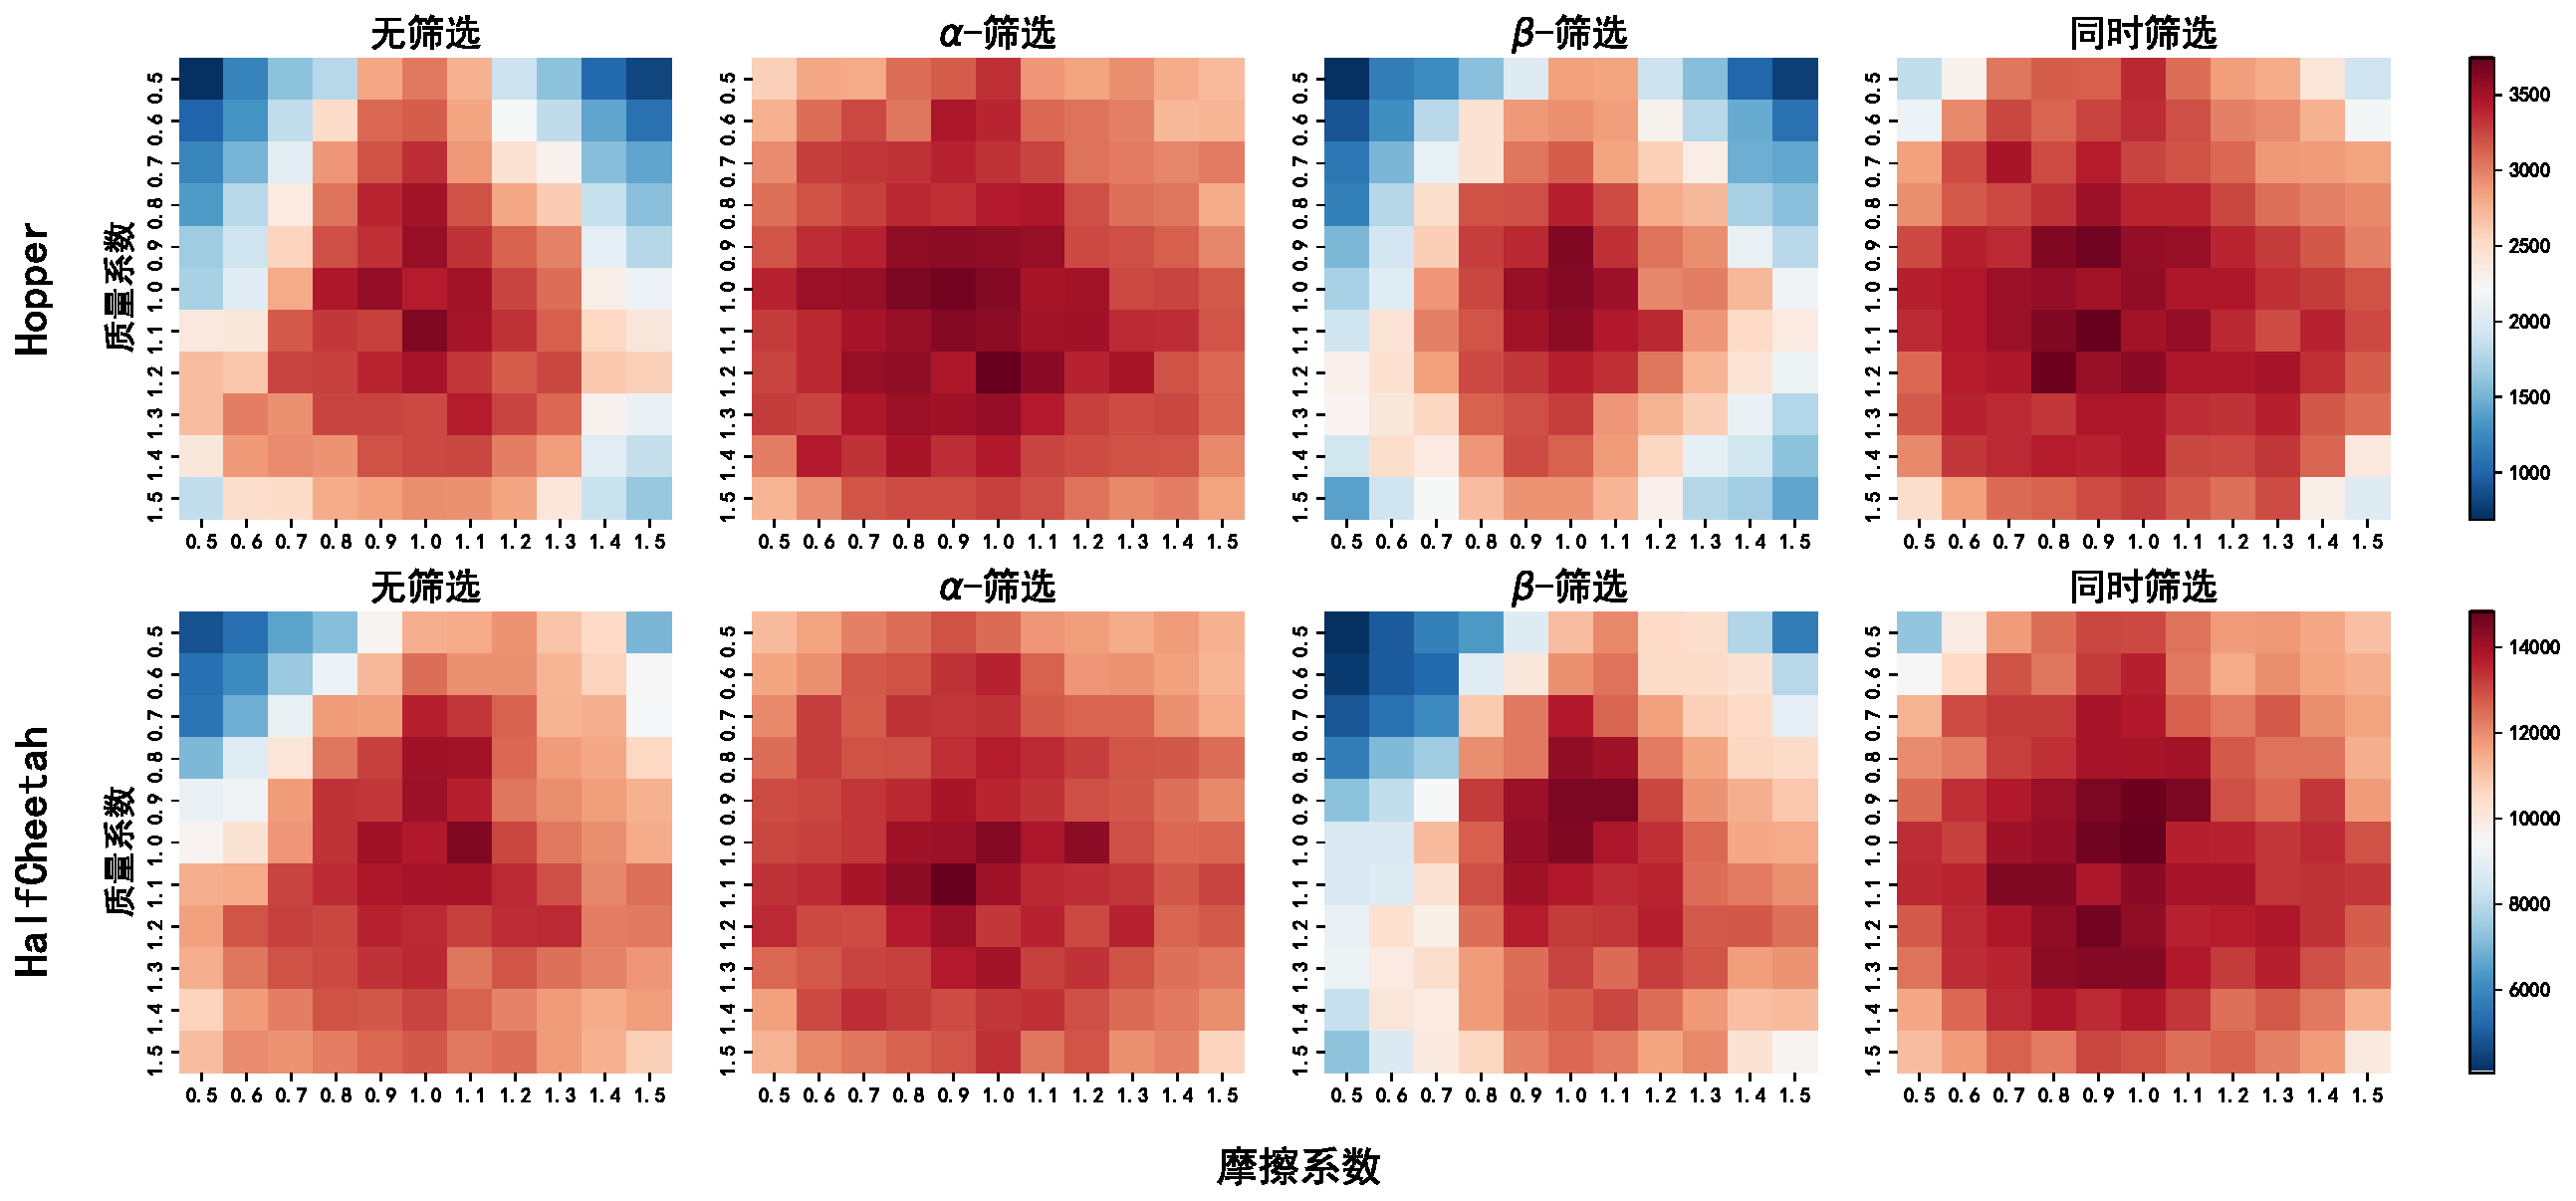
\includegraphics[width=0.7\textwidth]{figures/robustness-heatmap.pdf}
  \caption{算法鲁棒性对比实验。}
  \label{fig:robustness-heatmap}
\end{figure}

\section{自动化温室决策控制任务}
